\documentclass[10pt,a4paper]{report}
\usepackage[utf8]{inputenc}
\usepackage[english]{babel}
\usepackage[T1]{fontenc}
\usepackage{amsmath}
\usepackage{amsfonts}
\usepackage{amssymb}
\usepackage{listings} % code highlights
\usepackage{fancyhdr} % headers and footers
\usepackage{graphicx}
\usepackage[left=2.5cm,right=2.5cm,top=2.5cm,bottom=2.5cm]{geometry}
\usepackage[nottoc]{tocbibind}
\usepackage{setspace}
\usepackage{float}
\onehalfspacing

\author{Anuta Christian,Givron Azim}
\title{The aerodynamics of the frisbee}

% Hide chapters numbers 
\renewcommand{\thesection}{\arabic{section}}

% Set headers and footers
\pagestyle{fancy}
\fancyhf{}
\lfoot{MECA-H3001: fluid mechanics and transfer process}
\rfoot{ \thepage}
\renewcommand{\headrulewidth}{0pt}   % head horizontal rule 
\renewcommand{\footrulewidth}{0.5pt} % foot horizontal rule

\begin{document}

\begin{titlepage}
\noindent Université libre de Bruxelles
\\Informatics section
\\$3^{rd}$ year of study

\center 

\includegraphics[scale=0.5]{logo-polytech-ULB-FR.jpg}\\
\vspace{5cm}
\textsc{\large MECA-H3001} \\[0.5cm]
\textsc{\LARGE Fluid mechanics and transfer process} \\[1.5cm]
\textsc{\Large The aerodynamics of the frisbee} \\[1.5cm]
\rule{\textwidth}{1pt}

\vspace{0.5cm}
\textsc{\small Ms Kappel, Mr Parente and Mr Debaste} \\[0.5cm]
\textsc{\small The 14th December 2017} \\[0.5cm]

\rule{\textwidth}{1pt}

\vspace{2cm}

\textsc{\large Anuta Christian and Givron Azim}

\end{titlepage}

\tableofcontents
\newpage 
\listoffigures
\newpage
\section{Abstract}
Since the original 1963 Frisbee, flying discs have evolved becoming ubiquitous and far-ranging. Effects of drag and lift forces applied on those discs are analyzed in this project through simulations. They predict the flight trajectory of a disc in two dimensions based on the angle of attack and the initial velocity input parameters. Equations for the simulations came from the forces known to act on flying objects as well as coefficient functions for lift and drag. The results of the experiment show that the optimal angle of attack was about $10\,^{\circ}$, which is explainable by considering two phenomena : the lift and the recirculation region.
\section{Introduction}
The frisbee was invented decades ago. However we still use it today as a source of amusement for kids and grown-ups. It is not only used to entertain people, it also permits to create new sports such as the ultimate frisbee or the disc golf. This object has a particular shape which allows it to glide for really long distances but, to make the most of it the toss has to be well oriented. The optimal angle of the throw is precisely the object of this report. In order to determine it, we first need to understand the mechanisms that allows the frisbee to soar. In this purpose, we have to consider the constraints decree by the geometry of the frisbee and the fluid mechanics laws. Thus, on one hand, the frisbee's shape demands the air travelling above to be faster than the one below it\footnote{(Morrison V. R. 2005, 1-12), (Baumback et al. 2010, 1-16)}, while on the other hand, bernoulli's equation states \footnote{(\c{C}engel et al. 2006,562-601 )} that the pressure is low at locations where the flow velocity is high and vice-versa. Therefore the pressure exerted under the frisbee is higher than the one exerted above it. Consequently the frisbee can glide. Notice that the difference of pressure between both sides of the frisbee is due to a force pointing upward, normal to the flow direction and it is called the lift. 

\begin{figure}[H]
\centering
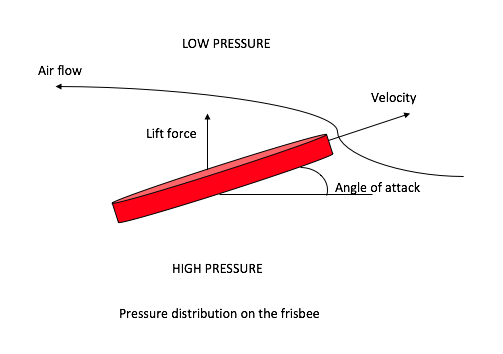
\includegraphics[scale=0.6]{Intro.jpg}
\caption{Pressure distribution on the frisbee}
\label{Pressure distribution on the frisbee}
\end{figure}

\section{Method}
In order to ascertain the optimal throw, we simulated the frisbee's trajectory by computing simulation. This requires to know the velocity and the position of the frisbee at anytime. Since the acceleration modify the velocity through time, we should thus calculate it. This is possible by using the second law of Newton $F = ma$ where $F$ is the force exerted on the body of mass $m$ and $a$ is its acceleration. It implies implicitly that we have to find the main forces acting on the frisbee,  which are the gravitational force and the lift and drag forces illustrated on the Figure ~\ref{Forces acting on the frisbee}. The latter is the force exerted by the air on the frisbee in the flow direction, it is the air resistance. Since these forces only act in parallel and perpendicularly to the flow, the simulation can be simplified by only considering those two dimensions.

\begin{figure}[H]
\centering
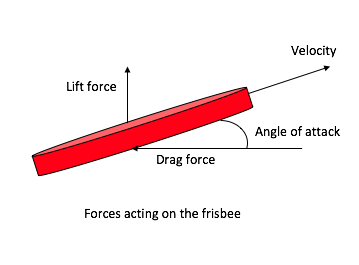
\includegraphics[scale=0.6]{forces.jpg}
\caption{Forces acting on the frisbee}
\label{Forces acting on the frisbee}
\end{figure}

\subsection{Mathematical description}
The three forces cited above are all expressed by physical relationships. In the following part, we will present these relationships.
\\The gravitational force $F_g$\footnote{(Baumback et al. 2010, 1-16)} applied on the frisbee is directly proportional to its mass $m$
\[F_g = m g\]
with $g$, the gravitational acceleration.
\\
The drag and lift forces are more difficult to find because the equations depend on the geometry of the object studied, and the object's direction in comparison to the fluid's one. Fortunately, the frisbee's geometry approximates the one of a flat plate. In this case, the drag and lift forces are respectively given by\footnote{(\c{C}engel et al. 2006,562-601 )} :
\[F_d = -\frac{C_d \rho A  v^2}{2}\]
\[F_l = \frac{C_l \rho A  v^2}{2}\]
In this particular case, the fluid is the air, thus $\rho$ is its density, $v$ is the velocity of the Frisbee relative to the air, A is the surface area of the plate exposed to the air flow and $C_d$ and $C_l$ are respectively the drag and lift coefficients.
The drag coefficient, generally, depends on the Reynolds number which gives the type of flow studied. A flow can be laminar or turbulent. The first one relates to ordered flows while the second one caracterise chaotics flows. This number can be calculated with the following relationship:
\[\Re = \frac{\rho v d}{\eta}\]
where the only new term appearing here is $\eta$, the viscosity of the air.
By using the data presented at the result section, we found $Re=2.59$ $10^5$ which correspond to a turbulent flow.
In this case, the drag coefficient can expressed as:
\[C_d = C_{d0} + C_{d\alpha}(\alpha-\alpha_0)^2\]
which links it to the angle of attack $\alpha$. The other terms are constants found experimentally\footnote{(Morrison V. R. 2005, 1-12), (Baumback et al. 2010, 1-16)}.
\\Finally, the lift coefficient can be found with the relationship below:
\[C_l = C_{l0} + C_{l \alpha} \alpha\]
where $C_{l0}$ and $C_{l\alpha}$ are also constants found by experiments.
\subsection{Numerical modelling}
Solving this problem numerically can be done by using different methods\footnote{(Schroeder 2015, 1-32)}. Here, we will use the Euler progressive method. It simply means that a position is calculated from the previous one\footnote{(Morrison V. R. 2005, 1-12)}.
The angle of attack appears in the initial conditions since it represents the angle of the toss. Thus, the variation of this angle will give us different graphs representing the frisbee's trajectory.
\section{Results}
In this section, we will present three graphs\footnote{(Baumback et al. 2010, 1-16)} that we obtained from the simulation. All of them were made with the same parameter values except for the angle of attack which is varying from $5\,^{\circ}$ up to $45\,^{\circ} $. 
\\The parameter values are the following:
\\
\begin{center}
\begin{tabular}{|l|c|r|}
  \hline
  Symbol & Signification & Value \\
  \hline
  $m$ & Mass of frisbee & 0.175 $kg$\\
  $\rho$ & The density of air & 1.23 $kg/m^3$\\
  $g$ & Acceleration of gravity & 9.81 $m/s^2$ \\
  $d$ & Diameter of Frisbee & 0.26 $m$ \\
  $A$ & Surface area of Frisbee & $\pi (d/2)^2$ $m^2$ \\
  $v_i$ & Initial velocity & 14 $m/s$ \\
  $v_x$ & Initial velocity in the x-direction & $v_icos(\alpha)$ $m/s$ \\
  $v_y$ & Initial velocity in the y-direction & $v_isin(\alpha)$ $m/s$ \\
  $C_{D0}$ & Frisbee dimensional constant & $0.08$ \\
  $C_{L0}$ & Frisbee dimensional constant & $0.15$ \\
  $\alpha_0$ & Frisbee dimensional constant & $-4\pi / 180$ $rad$ \\
  $C_{D\alpha}$ & Frisbee dimensional constant & $2.72$ $rad^{-2}$\\
  $C_{L\alpha}$ & Frisbee dimensional constant & $1.4 $ $rad^{-1}$\\
  \\
  \hline
\end{tabular}
\end{center}
\begin{figure}[H]
 \centering
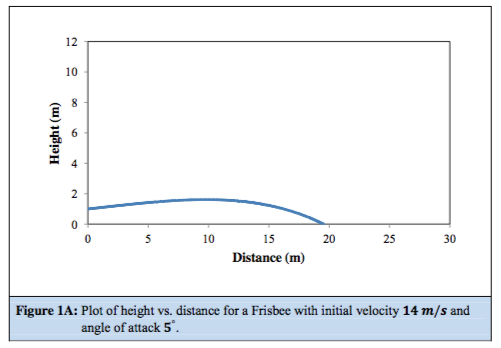
\includegraphics[scale=0.6]{graph1.jpg}
\caption{First result}
\label{First result}
\end{figure}
\leavevmode
\\The first graph (Figure ~\ref{First result}) shows that an angle of attack of $5\,^{\circ}$ permits the frisbee to reach a distance of $19m$.
\begin{figure}[H]
\centering
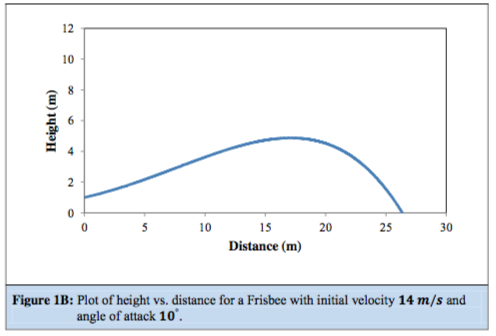
\includegraphics[scale=0.6]{graph2.jpg}
\caption{Second result}
\label{Second result}
\end{figure}
\leavevmode
\\The second one (Figure ~\ref{Second result}), thrown with an angle of $10\,^{\circ}$ travelled for $26m$.
\begin{figure}[H]
\centering
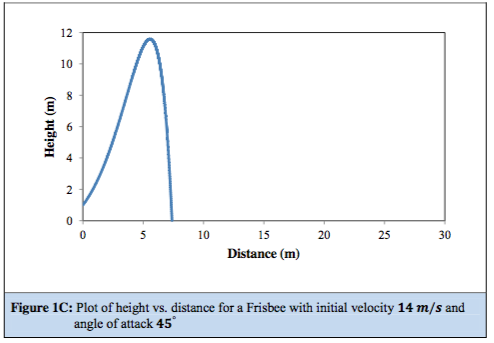
\includegraphics[scale=0.6]{graph3.jpg}
\caption{Third result}
\label{Third result}
\end{figure}
\leavevmode
\\The last one (Figure ~\ref{Third result}) only glide for $8m$ but was tossed with an angle of $45\,^{\circ} $.

\section{Discussion}
The different graphs show that the angle of attack has an important impact on the distance travelled by the frisbee. The best results were obtain with an angle of $10\,^{\circ}$ which is not an intuitive result. In fact we would rather think that a $45\,^{\circ}$ inclination would allow a higher lift, since this force is the vertical projection of the force applied on the frisbee by the flow. Thus the lower the angle would be(under$45\,^{\circ}$), the lower the lift would be. This is the idea shown on Figure ~\ref{Lift cause by the flow for different angle}.
\begin{figure}[H]
\centering
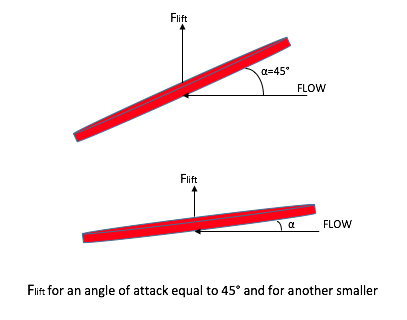
\includegraphics[scale=0.6]{intuitive.jpg}
\caption{Lift cause by the flow for different angles of attack}
\label{Lift cause by the flow for different angle}
\end{figure}
In reality, it is not the case and it is explainable by introducing the concept of recirculation region\footnote{(\c{C}engel et al. 2006,562-601 )}. When the frisbee's inclination is not null, there is a flow separation. This create two different areas at different pressures. The pressure difference forces the flow to come back in the region where the pressure is lower which is below the frisbee, and is called the recirculation region. This movement of air is opposed to the flow direction, thus it increases the drag force which slows down the frisbee. Therefore, the higher the angle is, the higher the drag is.
\\Then the optimal angle is nothing else than the result of those two phenomena.
\section{Conclusion}
Throughout the simulation the results appeared to be quite unexpected. It is only after a deep research trough fluid mechanics phenomena that we could understand them. More precisely there were two of them : the lift force and the recirculation region. The first one is simply due to the acceleration provided by the air flow, and allows the frisbee to gain altitude. The second one is caused by the inclination of the frisbee relative to the air velocity, and lead to an increase of the air resistance. From those physical concepts, we were able to understand that the angle of attack would be greater than $0\,^{\circ}$ but smaller than $45\,^{\circ}$, and it appeared to be optimal for a $10\,^{\circ}$ inclination.

\begin{thebibliography}{9}
  
  \bibitem{phd1}
  Morrison V. R.,
  2005,
  “The Physics of Frisbees”,
  PhD diss.,
  Mount Allison University,
  
  Morrison is a research scientist graduated from the Mount Allison university and is currently working at the Talmic Lab which is specialized in electronic compound. His thesis has probably been peer-reviewed.
	
 \bibitem{art1}
Peter Lissaman, Mont Hubbard, Maximum range of flying discs, In Procedia Engineering, Volume 2, Issue 2, 2010, Pages 2529-2535, ISSN 1877-7058, https://doi.org/10.1016/j.proeng.2010.04.027.
(http://www.sciencedirect.com/science/article/pii/S187770581000281X)
Keywords: Flying discs; Frisbee; Flight dynamics

Peter Lissaman has provided many other articles about object under turbulent phenomena. Mont Hubbard is working at the University of California in the department of Mechanical \& Aerospace Engineering which makes him authoritative. Procedia Engineering is an open access collection of conference proceedings published between 2012 and 2017, with an emphasis in core engineering disciplines, such as aerospace, chemical, civil, mechanical or structural engineering. This article is certainly peer-reviewed and up-to-date.
  
  \bibitem{art2}
Reno Koyanagi, Kazuya Seo, Ken Ohta, Yuji Ohgi, A computer simulation of the flying disc based on the wind tunnel test data, In Procedia Engineering, Volume 34, 2012, Pages 80-85, ISSN 1877-7058, https://doi.org/10.1016/j.proeng.2012.04.015.
(http://www.sciencedirect.com/science/article/pii/S1877705812016281)
Keywords: Flying disc; computer simulation; aerodynamics
  
  \bibitem{art3}
Baumback, Kathleen (2010) "The Aerodynamics of Frisbee Flight," Undergraduate Journal of Mathematical Modeling: One + Two: Vol. 3: Iss. 1, Article 19.
DOI: http://dx.doi.org/10.5038/2326-3652.3.1.31
Available at: http://scholarcommons.usf.edu/ujmm/vol3/iss1/31

In 2017, Undergraduate Journal of Mathematical Modeling: One + Two was awarded the DOAJ Seal for its high degree of openness and for adhering to best practices and high publishing standards. So this article is peer-reviewed and up-to-date.
  
  \bibitem{phd2}
Schroeder, Erynn J., "An Aerodynamic Simulation of Disc Flight" (2015). Honors Theses. 68.
http://digitalcommons.csbsju.edu/honors\_theses/68

It is a thesis that has been reviewed by a teacher (Dr. Thomas Kirkman). The code of his simulation is given in the annexe and there are many sources from scientific articles to University courses.
  
  \bibitem{book1}
  \c{C}engel, Yunus A., and John M. Cimbala. 2006. Fluid mechanics: fundamentals and applications. Boston: McGraw-HillHigher Education.
  
  This book is used by many teachers (including ours) and represent the basics of fluid mechanics. Thus, this is definitely a reliable source.

\end{thebibliography}
\end{document}